\documentclass[twocolumn]{article}

% Language setting
% Replace `english' with e.g. `spanish' to change the document language
\usepackage[english]{babel}

% Set page size and margins
% Replace `letterpaper' with`a4paper' for UK/EU standard size
% \usepackage[a4paper,top=2cm,bottom=2cm,left=3cm,right=3cm,marginparwidth=1.75cm]{geometry}

% Useful packages
\usepackage{amsmath}
\usepackage{amssymb}
\usepackage{amsfonts}
\usepackage{graphicx}
\usepackage[colorlinks=true, allcolors=blue]{hyperref}
\usepackage{subfig}
\usepackage{multirow}

% Portuguese text
\usepackage[utf8]{inputenc}
\usepackage[T1]{fontenc}
\usepackage{hyphenat}

\usepackage{fullpage}  % Full page
\usepackage{booktabs}  % Pandas output
\usepackage{microtype}  % Solve overfull
\usepackage{float}

\graphicspath{ {../images/} }

\title{Separability of legal documents according to precedent citations}
\author{Lucas Emanuel Resck Domingues \\
\large \textit{School of Applied Mathematics} \\
\textit{Getulio Vargas Foundation} \\
\textit{lucas.domingues@fgv.edu.br}}

\date{\today}

\newcommand{\ie}{\textit{i.e.}}
\newcommand{\eg}{\textit{e.g.}}

\begin{document}
      % https://tex.stackexchange.com/a/140679
      % https://tex.stackexchange.com/a/21126
      % https://tex.stackexchange.com/a/28110
      \twocolumn[
            \begin{@twocolumnfalse}
                  \maketitle
                  \begin{abstract}
                        The Brazilian Supreme Court (STF) frequently cites what is called a ``Súmula Vinculante,'' or Binding Precedent (BP), in their decisions, which is a precedent that has mandatory application. 58 BPs were have already been created until today. It seems trivial that documents that cite the same precedents have the same subjects, and documents that cite different precedents have different subjects. In this work, we explore if this is also trivial for machine learning models, \ie, if traditional machine learning models can learn to ``separate'' these documents according to precedent citations, particularly Binding Precedents. We begin with an exploration of our dataset; we explain the methodology of the experiments; we adjust several supervised and unsupervised models; we discuss the results. The main result is the fact that the documents are very separable, even linearly separable, according to the BP citations.
                  \end{abstract}
            \end{@twocolumnfalse}
            \bigskip
      ]

      \section{Introduction}

    The Brazilian Supreme Court (STF) is the highest law court in Brazil. It produces a large number of documents during its functioning, \eg, more than 1 million STF decisions were produced between 2011 and 2020 \cite{stf}. STF is not the only institution that deals with overload: it is spread all over the Brazilian Judicial System.

    One approach to solving this overload problem is the so-called precedent: when a similar case has to be decided again, this new decision can be taken based on the referenced old decision. This way, cases are solved faster. Many precedents about a subject in a court are consolidated in a ``súmula'', a document that resumes the court's understanding about that subject. However, the application of this understanding is not mandatory, and the judge can take a different decision. This situation can lead not only to judicial inefficiency but also to judicial insecurity: similar cases with different results.

    With this situation in mind, STF was allowed, in 2004, by Constitutional Amendment, to create ``Súmulas Vinculantes'', which we will call here ``Binding Precedents'', or just BPs. They are the old súmulas, but with mandatory application. These BPs are frequently cited in STF decisions.

    It seems trivial that documents that cite the same precedents have the same subjects, and documents that cite different precedents have different subjects, in general. However, can machine learning models and algorithms identify this pattern themselves? That is, if a trained machine learning model is presented to a document, can it predict which precedent is being cited? These questions are very relevant because, if the answer is positive, artificial intelligence algorithms can assist legal experts during their analysis, considering that legal documents many times are long and in large numbers.

    This situation of predicting the correct precedent is what is being called here as ``separability'' of documents as if the documents could be separable in high dimensional space. In this assignment, this separability will consider Binding Precedents in STF decisions. This work is organized as follows. In \autoref{sec:dataset}, we describe the BPs, our dataset, and we also make a short data exploration. In \autoref{sec:methodology}, we present the methodology that will be followed in our experiments with machine learning models, briefly introducing these models, and presenting some details that weren't covered during the course. In \autoref{sec:results}, we show the experiment results and a discussion about what was found.


      \section{Dataset}
      \label{sec:dataset}

      \subsection{Binding Precedents}

            Until June 2021, 58 Binding Precendents have already been created. For example, take a look at BP 10's statement:

            \textit{``Viola a cláusula de reserva de plenário (CF, artigo 97) a decisão de órgão fracionário de tribunal que, embora não declare expressamente a inconstitucionalidade de lei ou ato normativo do Poder Público, afasta sua incidência, no todo ou em parte.''}
            
            The statements are short, in general, but in legal language (and in Portuguese). Although it can lead to some insights, we are not interested in studying the meaning of BP's statements.

      \subsection{Dataset description}

            The dataset used throughout this work is composed of decisions generated by STF that cite at least one Binding Precedent. Although these documents are public, they are very difficult to be accessed, mainly when it is necessary a large amount of data. This way, we use a dataset gathered in the context of Supremo em Números project \cite{falcao2013relatorio}, from FGV's Law School.

            The dataset, in the way we have it, is composed of 58 CSV files of structured data, with columns:
            \begin{itemize}
                  \item \textit{title}: document title, formed by date, document type, and an ID;
                  \item \textit{raw\_text}: document's raw text;
                  \item \textit{i\_cite}: list of cited precedents, including BPs, already extracted from the raw texts;
                  \item \textit{date}: document's publication date.
            \end{itemize}

            This is how a usual document looks like:

            \bigskip

            {\itshape``DECISÃO

            AGRAVO DE INSTRUMENTO. PROCESSUAL CIVIL. PERDA SUPERVENIENTE DO OBJETO. RECURSO ESPECIAL PROVIDO PARA ANULAR O ACÓRDÃO RECORRIDO. AGRAVO DE INSTRUMENTO PREJUDICADO.

            Relatório

            1. Agravo de instrumento contra decisão que não admitiu recurso extraordinário interposto com base no art. 102, inc. III, alínea a, da Constituição da República. (...)''}

      \subsection{Exploratory data analysis}

            Although our dataset is very simple (few, self-explanatory columns), we can analyze it more deeply to better understand it. Let's start, for example, by checking how many citations each BP has.

            \begin{figure}[H]
                  \centering
                  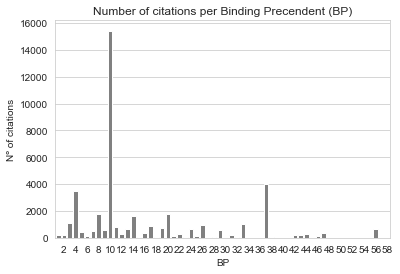
\includegraphics[width=\linewidth]{bp_citations.png}
                  \caption{Histogram of citations per Binding Precedent.}
                  \label{fig:bp_citations}
            \end{figure}

            From \autoref{fig:bp_citations}, we see that the number of citations per BP is not uniform. BP 10, for example, has the largest number of citations, followed by 37, 4, and 8. This large difference in the citation number can impact our analysis if we don't work around it.

            We already know the documents are long, but one could want to know how long these documents are. If we split each document at whitespaces and newlines and count the number of ``words'', we have a document word count distribution estimate.

            \begin{figure}[H]
                  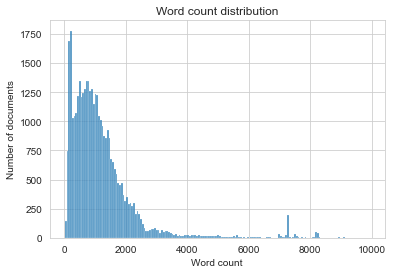
\includegraphics[width=\linewidth]{word_count.png}
                  \caption{Estimate of document word count distribution.}
                  \label{fig:word_count}
            \end{figure}

            There are some special documents (more than 10k words), but their analysis is not our focus. \autoref{fig:word_count} shows that, in general, documents are shorter than 6k words, with a mode around 1k.

            Although document titles are unique, many documents share the same raw text. This ``duplicate'' rate is around 11\%, and can also impact our subsequent analyses. This way, we need to work around these duplicated documents before fitting our models.

            Finally, one could want to see the distribution of publication date, presented in \autoref{fig:dates}. Date distribution has support between 2003 and 2018 (not clear in the plot), but it is concentrated between 2008 and 2018. It is clear that many documents have the publication year 1970, however, this information acts as a missing value. Although this is problematic, that is, many documents do not have a publication date, it will not impact our models, because we only work with raw texts.

            \begin{figure}[H]
                  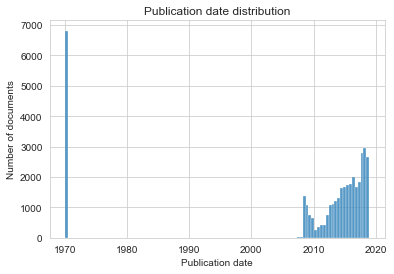
\includegraphics[width=\linewidth]{dates.png}
                  \caption{Distribution of document publication date.}
                  \label{fig:dates}
            \end{figure}
            

      \section{Methodology}
    \label{sec:methodology}

    \subsection{Document embedding}
    \label{sec:document_embedding}

    \paragraph{TF-IDF.} Before texts can be fed into machine learning models, they need to become numbers, usually vectors. These vectors are called text embeddings, and, in the case of long documents, document embeddings. There are many document embedding techniques available, but, for the scope of this work, we will use here TF-IDF \cite{robertson2004understanding}.

    Briefly, for each document, and for each word, TF-IDF counts the frequency of this word relative to this document (term frequency - TF). This count is ``normalized'' by the rarity of the word in the entire set of documents (inverse document frequency - IDF). Mathematically, for a term $t$ inside document $d$ with frequency $f_{t, d}$,
    \[\text{tf-idf}(t, d) = \text{tf}(t, d) \times \text{idf}(t),\]
    \[\text{tf}(t, d) = \frac{f_{t, d}}{\sum_{t' \in d} f_{t', d}}, \ \ \text{idf}(t) = \ln \frac{1+n}{1+\text{df}(t)}+1,\]                  
    where $n$ is the number of documents and $\text{df}(t)$ is the number of documents that contain $t$. The TF-IDF weights, in the end, construct a vector that represents the document in a very high dimensional space.

    \paragraph{Dimensionality reduction.} Because vectors' dimensionality is too high, we perform a dimensionality reduction to have the vectors treatable by our models. The vectors will be reduced from dimensionality of thousands to dimensionality 50 using truncated singular value decomposition (SVD). It consists of decomposing our matrix $X$ (with rows being the TF-IDF vectors) in
    \[X = U \Sigma V^\intercal,\]                  
    where $\Sigma$ is a diagonal matrix of the singular values of $X$. If we take only the $k$ greatest singular values, we will have
    \[X_{n \times p} = U_{n \times k} \Sigma_{k \times k} \left[V^\intercal\right]_{k \times p},\]                  
    and our new data points will be $X_{n \times p} V_{p \times k}$, with reduced dimensionality $k$. This is very similar to principal component analysis, and equivalent when data is centered (mean zero in each component).



    \subsection{Text preprocessing}

    Our texts need to be preprocessed before being converted into TF-IDF vectors. One motivation of this preprocessing is the fact that we are not interested in the weights of the words ``the'', ``to'', and ``that'', for example.

    The preprocessing pipeline adopted in our work considers:
    \begin{itemize}
    \item Lowercase: convert the documents into lowercase;
    \item Tokenize: split the documents into tokens (``words'');
    \item Lemmatization: convert a token to its ``lemma'', \ie, the dictionary version of this token;
    \item Remove stopwords: tokens such as ``the'';
    \item Remove punctuation.
    \end{itemize}


    \subsection{Machine learning models}
    \label{sec:models}

    The main goal of this work is to assert whether traditional machine learning models can ``separate'' documents according to BP citations. We will explore two approaches: unsupervised and supervised learning, with a focus on the latter.

    Unsupervised learning means extracting patterns from data that is not labeled, \eg, our raw documents. Considering this, we will present the raw documents to some algorithms, without explaining which precedents are being cited, and we will check their outputs to see if there is some pattern.

    We have vectors representing our texts as $X$ and cited BPs as $y$, the definition of supervised learning. With this in mind, we will also adjust several supervised models in this data.

    \paragraph{Latent Dirichlet allocation.} Because we are dealing with texts, it is very convenient to experiment with latent Dirichlet allocation (LDA), the most common topic modeling technique. Assuming the existence of $K$ topics, each document has a distribution over the topics, and each topic has a distribution over the words. Mathematically, the formulation is:

    \begin{itemize}
            \item Each topic $k \in \{1, \cdots, K\}$ has distribution $\beta_k \sim \text{Dirichlet}(\eta)$ over the words;
            \item Each document $d \in \{1, \cdots, D\}$ has distribution $\theta_d \sim \text{Dirichlet}(\alpha)$ over the topics;
            \item Given a document $d$, the topics have distribution $z | \theta_d \sim \text{Multinomial}(\theta_d)$;
            \item Given a topic $k$, the words have distribution $w | \beta_k \sim \text{Multinomial}(\beta_k)$.
    \end{itemize}

    The idea of using this model is to verify whether LDA can recover the topic of the BP being cited in a document. For example, if there were only two cited precedents on the dataset, one could fit LDA using two topics and verify if the most important words for each topic are representative of the precedents themselves. Even more, it would be possible to verify if this topic to precedent assignment is good.

    \paragraph{Truncated SVD dimensionality reduction.} We will reduce the dimensionality of TF-IDF vectors to visualize if they are of some kind separable. The dimensionality reduction technique will be the (truncated) singular value decomposition, already explained in \autoref{sec:document_embedding}. We will experiment with dimensionalities 2 and 3, which can be visualized on a 2-dimensional screen.

    \paragraph{K-nearest neighbors.} As TF-IDF vectors lie in some vector space, the decision of each BP is being cited could be taken considering the already known precedent cited by its neighbor. This is what the k-nearest neighbors (k-NN) model does. The number of neighbors (parameter $k$) is chosen by cross-validation.

    \paragraph{Linear regression.} This model is already well known, but for regression. For classification, and when the target is binary, it is easy to fit a regression model using $y \in \{-1, 1\}$ and considering the predicted class as the prediction sign. For multiclass, it is fitted one regression per target, and the class with the highest value is chosen. We will also use Ridge regularization, and the hyperparameter is chosen by cross-validation.

    Although using linear regression for classification is not that convenient, mainly because the output can't be interpreted as a probability, we can use this model to assert if our vectors are \textbf{linearly separable} in the very high dimensional space.

    \paragraph{Logistic regression.} Logistic regression is like a linear regression for classification, so it is more suitable for our task. For adjusting the model for various classes, we will minimize the multinomial logistic regression loss \cite{bishop2006pattern}:
    \[- \sum_{n=1}^N \sum_{k=1}^K y_{nk} \ln p_{nk},\]                  
    $y_{nk}$ indicating that the sample $n$ belongs to class $k$, $p_{nk}$ the estimated probability of sample $n$ belonging to class $k$ (calculated with softmax of linear functions of $X_n$). We also experiment with $\ell^2$ regularization, chosen by cross-validation.

    \paragraph{Linear discriminant analysis.} Linear discriminant analysis fits a probability distribution for each class, considering the priori as the proportion of that class and the distribution of data, given the class, as a multivariate Gaussian. The decision boundary is linear, so we can also assert the \textbf{linear separability} of the documents.

    \paragraph{Random forest.} From decision tree models, we experiment with random forests. Just like a decision tree, but many of them aggregated, each considering a bootstrap sample of the dataset and also a sample of the predictors. For a regression task, we have learned that, when the decision space is divided into various nodes, the output of the model is the mean of the samples inside that node.

    It is natural to extend regression decision trees to classification decision trees. For example, with the already adjusted model, the predicted class is the class with more samples inside the node, and the probabilities are the class sample proportions.

    There are some hyperparameters to be chosen, \eg, depth of the trees and number of trees. These are chosen using cross-validation.

    \paragraph{Support vector machines.} Support vector machines (SVM) are very powerful, even having a simple mathematical formulation. Intuitively, they fit an optimal hyperplane dividing a transformation of the dataset, but also allowing some points to not obey this restriction. The optimization problem is:
    \[\begin{aligned}
        \min_{w, b, \zeta} \quad & \frac{1}{2}w^\intercal w + C \sum_{i = 1}^{N}{\zeta_i} \\
        \textrm{s.t.} \quad & y_i (w^\intercal \phi(x_i) + b) \ge 1 - \zeta_i \\
        & \zeta_i \ge 0, \ \ i = 1, \cdots, n. \\
    \end{aligned}\]
    The regularization $C$ parameter is chosen by cross-validation. The kernel function also is chosen by CV, between linear and radial basis function (RBF), so as the $\gamma$ hyperparameter of RBF.


    \subsection{Dataset split}

    Because the original dataset is very unbalanced among the Binding Precedent citations, we need to create a sample dataset that will be used in our analysis. In this sample, each document cites only one BP, to avoid confusion; documents that share the same raw texts are removed, to avoid overfitting; we only work with the five most cited BPs, for simplicity and also data limitation; the dataset is balanced among the classes, i.e., each class has the same number of documents. In the end, we work with 1401 documents of BPs 10, 37, 4, 20, and 14, totalizing 7005 documents. These are the five considered Binding Precedent texts:

    \begin{itemize}
            \item \textbf{Binding Precedent 4}: \textit{``Salvo nos casos previstos na Constituição, o salário mínimo não pode ser usado como indexador de base de cálculo de vantagem de servidor público ou de empregado, nem ser substituído por decisão judicial.''}
            \item \textbf{Binding Precedent 10}: \textit{``Viola a cláusula de reserva de plenário (CF, artigo 97) a decisão de órgão fracionário de tribunal que, embora não declare expressamente a inconstitucionalidade de lei ou ato normativo do Poder Público, afasta sua incidência, no todo ou em parte.''}
            \item \textbf{Binding Precedent 14}: \textit{``É direito do defensor, no interesse do representado, ter acesso amplo aos elementos de prova que, já documentados em procedimento investigatório realizado por órgão com competência de polícia judiciária, digam respeito ao exercício do direito de defesa.''}
            \item \textbf{Binding Precedent 20}: \textit{``A Gratificação de Desempenho de Atividade Técnico-Administrativa - GDATA, instituída pela Lei 10.404/2002, deve ser deferida aos inativos nos valores correspondentes a 37,5 (trinta e sete vírgula cinco) pontos no período de fevereiro a maio de 2002 e, nos termos do artigo 5º, parágrafo único, da Lei 10.404/2002, no período de junho de 2002 até a conclusão dos efeitos do último ciclo de avaliação a que se refere o artigo 1º da Medida Provisória 198/2004, a partir da qual passa a ser de 60 (sessenta) pontos.''}
            \item \textbf{Binding Precedent 37}: \textit{``Não cabe ao Poder Judiciário, que não tem função legislativa, aumentar vencimentos de servidores públicos sob o fundamento de isonomia.''}
    \end{itemize}

    The main goal of this work is to assert whether traditional machine learning models can ``separate'' documents according to BP citations. For supervised learning models (predicting BP based on the raw text), we will create two datasets, training and test datasets, that will be used to fit and test these supervised models, respectively. Important to say that TF-IDF and truncated SVD (\autoref{sec:document_embedding}) are only fitted in training data, to guarantee generalization. The vectors also suffer a standardization (fitted in training data), as required by some supervised models.

    Several models need us to choose their hyperparameters, e.g., support vector machine (\autoref{sec:models}). For choosing a hyperparameter of a model, we perform K-fold cross-validation in the training dataset, i.e., for each hyperparameter, training data is split into $K$ sets, and, for each set $k$, the model is fitted in all other sets and validated in set $k$; the performances are aggregated. The hyperparameter with the best performance is the winner.


    \subsection{Performance metrics}

    Most of our algorithms are supervised and multiclass. The most suitable performance metric is the test accuracy, basically the ratio between hits and tries. We also present some test intraclass metrics, such as class precision (the fraction of BP $k$ predicted documents that are correct, for some BP $k$) and class recall (the fraction of correct BP $k$ documents that were predicted, for some BP $k$). In general, we also present a test confusion matrix, which shows how many test documents were predicted in each class.


    \subsection{Implementation}

    The models were implemented in Python, using the Scitkit-learn library, with the assistance of NumPy. Text preprocessing was done using the spaCy library, and graphics were plotted using Matplotlib, Seaborn, and Plotly libraries. The implementation is available at \href{https://github.com/lucasresck/machine-learning/}{https://github.com/lucasresck/machine-learning/} and can be better visualized \href{https://nbviewer.jupyter.org/github/lucasresck/machine-learning/blob/main/notebooks/a2_assignment.ipynb}{here}.

    

      \section{Results and discussion}
    \label{sec:results}

    \subsection{Latent Dirichlet allocation}

        Latent Dirichlet allocation was adjusted in our documents using five topics (components), the number of precedents we are considering. \autoref{fig:lda_topics} shows the top-20 words for each topic. From the barplot, we can see the following topics associated with the following BPs, justified by the following words:
        \begin{itemize}
                \item topic 1 \& BP 20: gratificação, inativos, atividade, desempenho, avaliação, gdata;
                \item topic 3 \& BP 4: salário, base, decisão, mínimo, constituição, cálculo;
                \item topic 4 \& BP 10: decisão, tribunal, constitucional, 10;
                \item topic 5 \& BP 14: acesso, direito, penal, inquérito, defeso, 14.
        \end{itemize}

        \begin{figure*}[!h]
                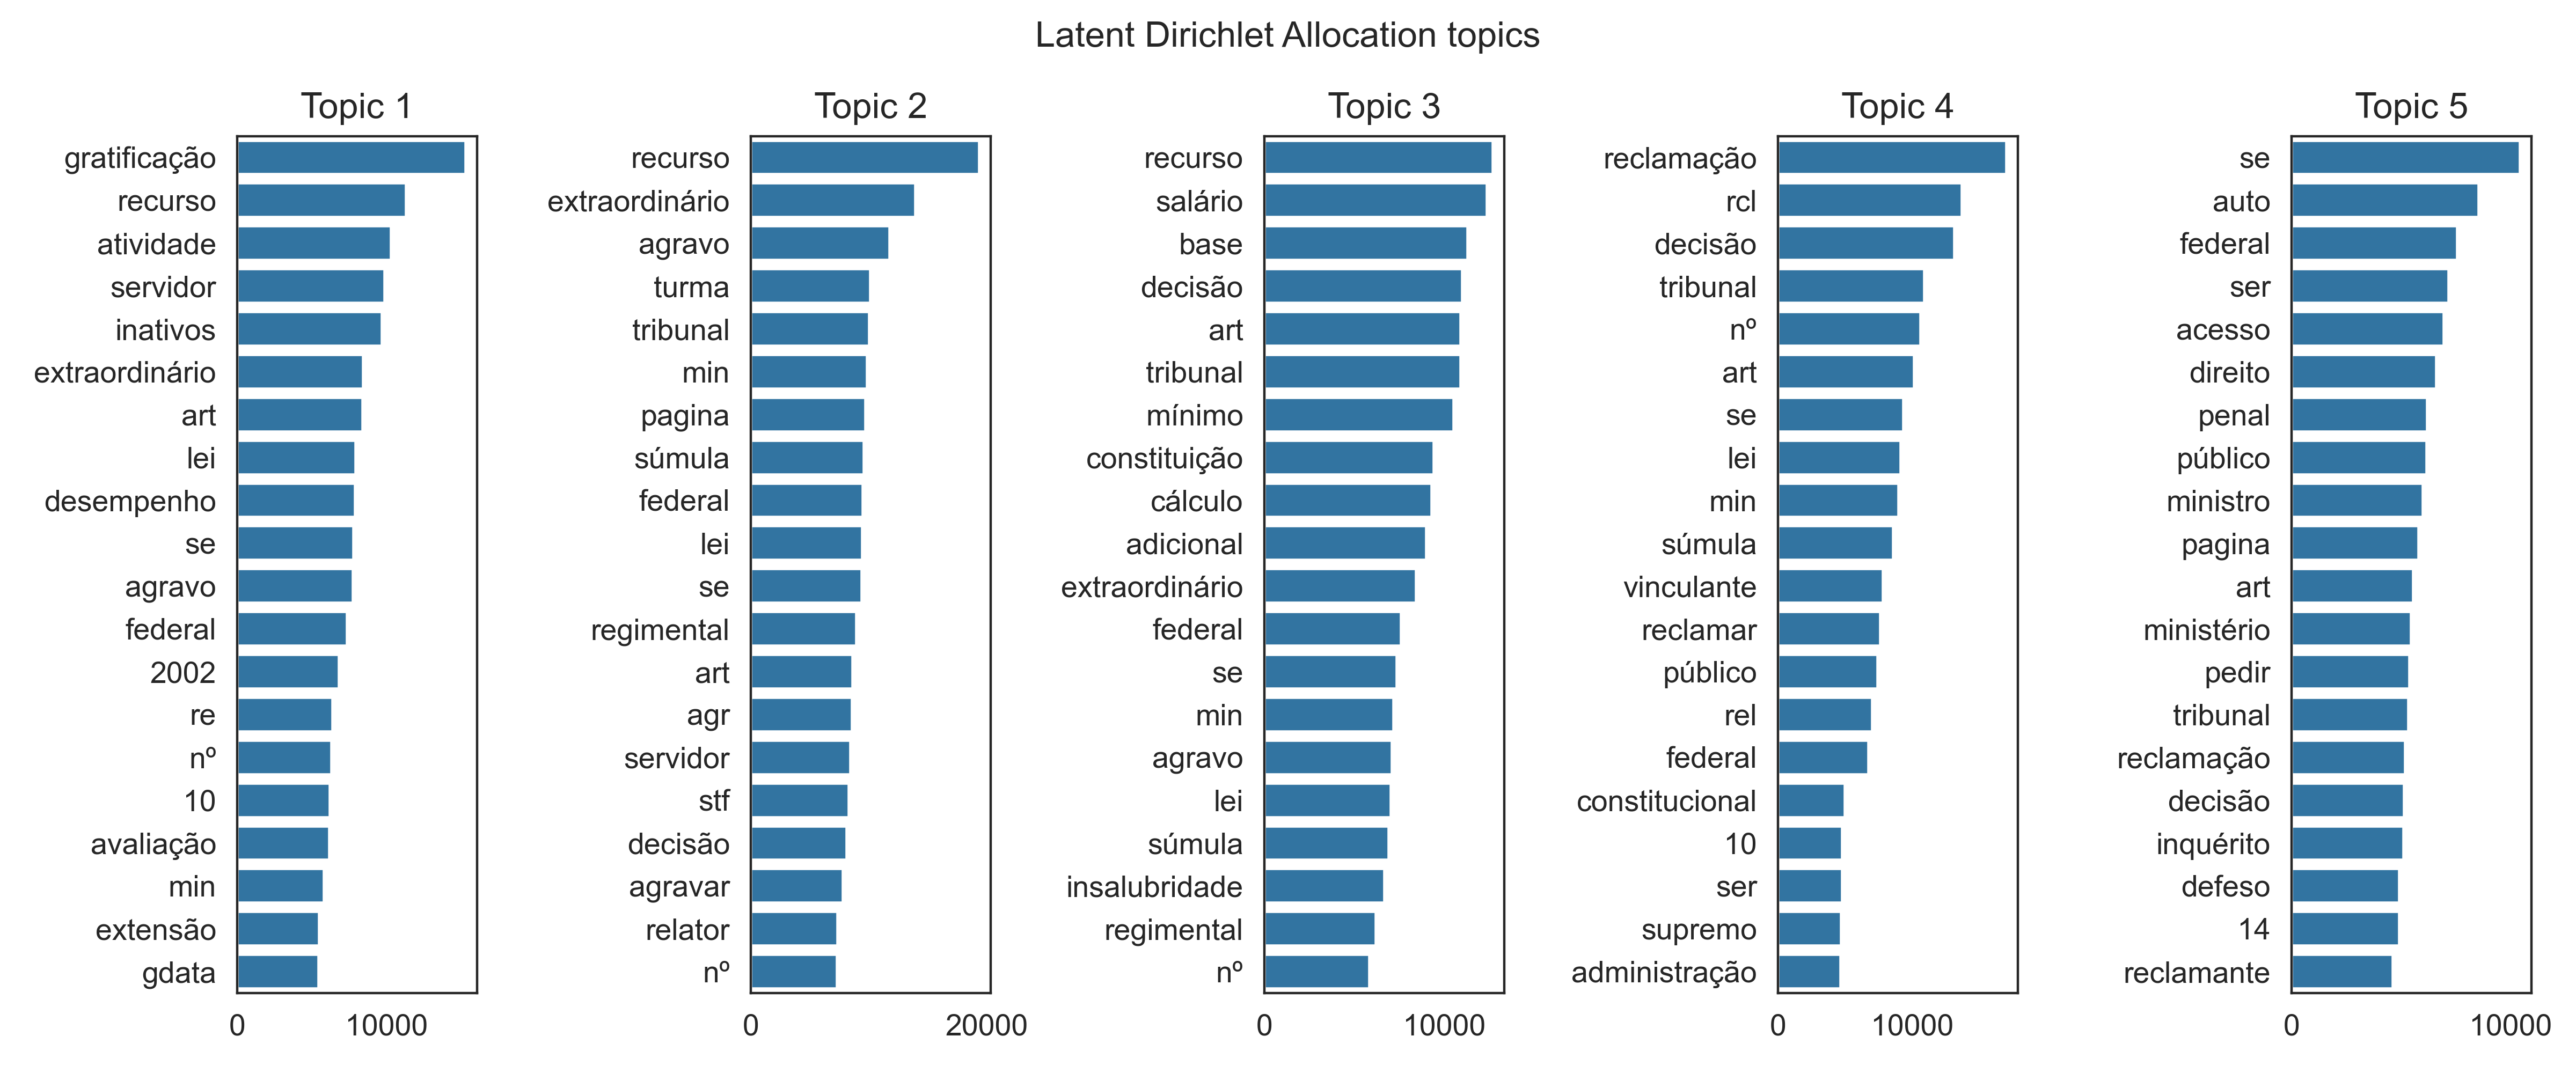
\includegraphics[width=\linewidth]{lda_topics.png}
                \caption{Top-20 words for each topic estimated with latent Dirichlet analysis.}
                \label{fig:lda_topics}
        \end{figure*}

        We can verify if the ``predicted'' topics match the real BPs being cited. Using this topic-to-BP assignment presented before, we get an accuracy of 0.76. That is, this topic modeling predicts the cited precedent correctly in 76\% of documents. We would expect 0.2 if it were a random assignment. So, LDA can extract the subjects of the BPs being cited.

    \subsection{Truncated SVD dimensionality reduction}

        \autoref{fig:svd_1} shows the resulting truncated SVD dimensionality reduction to 2. The color indicates the cited precedents, but the algorithm did not know that. We can see a pattern of data distribution, indicating that documents that cite the same BP are near each other.

        \begin{figure}[H]
                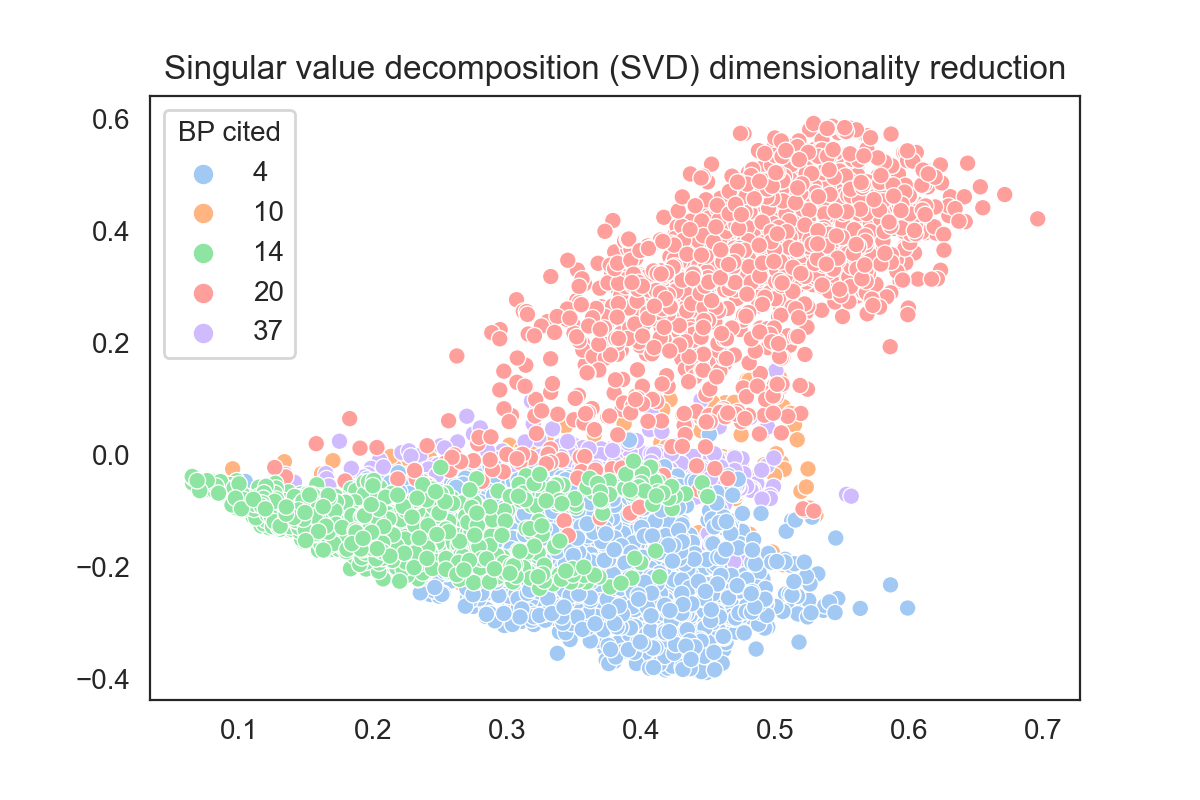
\includegraphics[width=\linewidth]{svd_1.png}
                \caption{Truncated singular value decomposition (SVD) dimensionality reduction to 2.}
                \label{fig:svd_1}
        \end{figure}

        \autoref{fig:svd_2_3}(a) and (b) present the result of dimensionality reduction to 3 dimensions. This graphic complements the last graphic, in the sense that it is more clear from this plot the fact that the documents can be separable in high dimensional space according to precedent citations.

        \begin{figure*}[!h]
                \centering
                \subfloat[\centering ]{{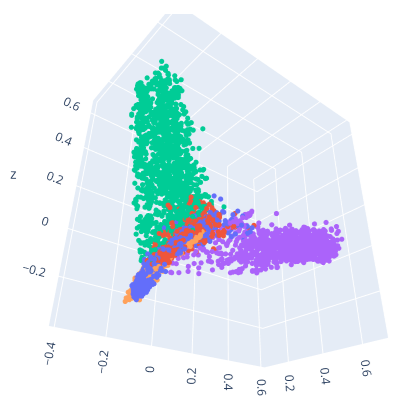
\includegraphics[width=0.4\linewidth]{svd_2.png} }}
                \qquad
                \subfloat[\centering ]{{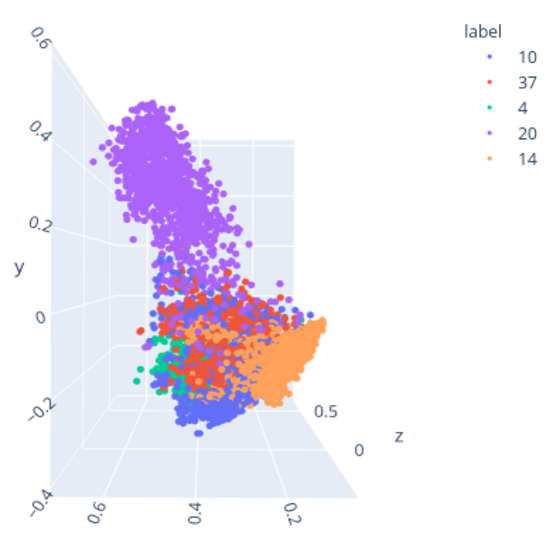
\includegraphics[width=0.4\linewidth]{svd_3.png} }}
                \caption{Truncated singular value decomposition (SVD) dimensionality reduction to 3.}
                \label{fig:svd_2_3}
        \end{figure*}

    \subsection{Linear regression}

        The results of classification using linear regression are presented in \autoref{tab:ridge}. Cross-validation to choose the Ridge regularization parameter was performed. All test metrics, \ie, precision, recall, and accuracy, are very high, which indicates the data is \textbf{linear separable}. \autoref{fig:rigde} shows the test confusion matrix, presenting how many documents from each BP were predicted as each BP. It is almost a diagonal matrix, indicating a very well-adjusted model.

        % Please add the following required packages to your document preamble:
        % \usepackage{multirow}
        \begin{table}[H]
                \centering
                \caption{Linear regression test metrics.}
                \label{tab:ridge}
                \begin{tabular}{c|cc|c}
                BP & Precision & Recall & Accuracy              \\ \hline
                4  & 0.96      & 0.91   & \multirow{5}{*}{0.95} \\
                10 & 0.94      & 0.93   &                       \\
                14 & 0.94      & 0.99   &                       \\
                20 & 0.99      & 0.95   &                       \\
                37 & 0.90      & 0.95   &                      
                \end{tabular}
        \end{table}

        \begin{figure}[H]
                \centering
                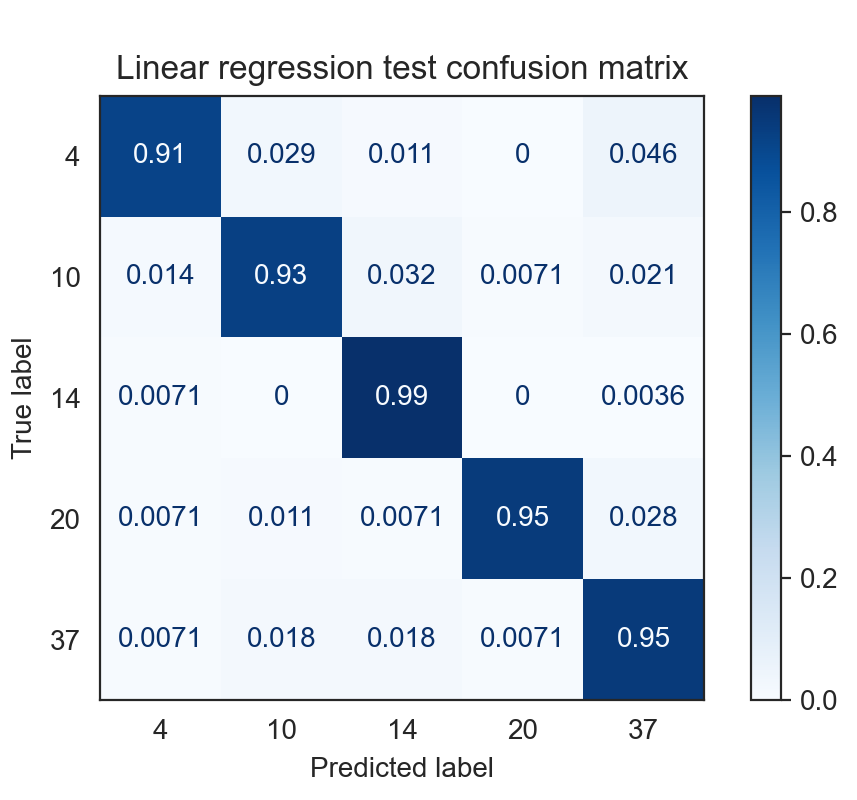
\includegraphics[width=0.8\linewidth]{ridge.png}
                \caption{Linear regression test confusion matrix.}
                \label{fig:rigde}
        \end{figure}

    \subsection{Logistic regression}

        \autoref{tab:lr} presents the results of classification using logistic regression. Cross-validation to choose $C$ regularization parameter was performed. All test metrics, \ie, precision, recall, and accuracy, are very high. Comparing to linear regression, the accuracy is even higher. \autoref{fig:lr} (in \autoref{sec:confusion_matrices}, from now on) shows the test confusion matrix. It is also almost a diagonal matrix, indicating a very well-adjusted model.

        % Please add the following required packages to your document preamble:
        % \usepackage{multirow}
        \begin{table}[H]
                \centering
                \caption{Logistic regression test metrics.}
                \label{tab:lr}
                \begin{tabular}{c|cc|c}
                BP & Precision & Recall & Accuracy              \\ \hline
                4  & 0.98      & 0.97   & \multirow{5}{*}{0.97} \\
                10 & 0.96      & 0.96   &                       \\
                14 & 0.98      & 0.99   &                       \\
                20 & 0.97      & 0.97   &                       \\
                37 & 0.95      & 0.96   &                      
                \end{tabular}
        \end{table}

    \subsection{Linear discriminant analysis}

        The results of classification using linear discriminant analysis are presented in \autoref{tab:lda}. All test metrics, \ie, precision, recall, and accuracy, are very high, which indicates the data is \textbf{linearly separable}. \autoref{fig:lda} shows the test confusion matrix, almost a diagonal matrix.

        % Please add the following required packages to your document preamble:
        % \usepackage{multirow}
        \begin{table}[H]
                \centering
                \caption{Linear discriminant analysis test metrics.}
                \label{tab:lda}
                \begin{tabular}{c|cc|c}
                BP & Precision & Recall & Accuracy              \\ \hline
                4  & 0.97      & 0.91   & \multirow{5}{*}{0.95} \\
                10 & 0.91      & 0.95   &                       \\
                14 & 0.97      & 0.99   &                       \\
                20 & 0.99      & 0.93   &                       \\
                37 & 0.90      & 0.96   &                      
                \end{tabular}
        \end{table}

    \subsection{K-nearest neighbors}

        \autoref{tab:k_nn} presents the results of using k-nearest neighbors for classification. For choosing the number $k$ of neighbors, it was performed cross-validation, and the chosen hyperparameter was $k = 1$. Test metrics, \ie, precision, recall, and accuracy, are high. \autoref{fig:k_nn} shows the test confusion matrix, which indicates high performance.
        
        % Please add the following required packages to your document preamble:
        % \usepackage{multirow}
        \begin{table}[H]
                \centering
                \caption{K-nearest neighbors test metrics.}
                \label{tab:k_nn}
                \begin{tabular}{c|cc|c}
                BP & Precision & Recall & Accuracy              \\ \hline
                4  & 0.93      & 0.95   & \multirow{5}{*}{0.93} \\
                10 & 0.87      & 0.90   &                       \\
                14 & 0.95      & 0.96   &                       \\
                20 & 0.97      & 0.95   &                       \\
                37 & 0.92      & 0.90   &                      
                \end{tabular}
        \end{table}

    \subsection{Random forest}

        The results of using a random forest for classification are shown in \autoref{tab:rf}. Hyperparameters of maximum tree depth and the number of estimators were chosen using cross-validation, resulting in no maximum depth and number of trees equal to 100. From test metrics, we see a very high performance. The test confusion matrix is also excellent, almost a diagonal matrix (\autoref{fig:rf}).
        
        % Please add the following required packages to your document preamble:
        % \usepackage{multirow}
        \begin{table}[H]
                \centering
                \caption{Random forest test metrics.}
                \label{tab:rf}
                \begin{tabular}{c|cc|c}
                BP & Precision & Recall & Accuracy              \\ \hline
                4  & 0.98      & 0.96   & \multirow{5}{*}{0.96} \\
                10 & 0.91      & 0.95   &                       \\
                14 & 0.98      & 0.99   &                       \\
                20 & 0.98      & 0.96   &                       \\
                37 & 0.94      & 0.93   &                      
                \end{tabular}
        \end{table}

    \subsection{Support vector machine}

        Test metrics relative to support vector machine used for classification are presented in \autoref{tab:svm}. From the metrics, we see very high performance in test data. The hyperparameters, which includes kernel function (linear vs. RBF), regularization parameter $C$, and $\gamma$, were chosen by CV, and the result was $C = 100$, $\gamma = 0.001$, and kernel RBF. The test confusion matrix is excellent, which indicates a very high model performance (\autoref{fig:svm}).
        
        % Please add the following required packages to your document preamble:
        % \usepackage{multirow}
        \begin{table}[H]
                \centering
                \caption{Support vector machine test metrics.}
                \label{tab:svm}
                \begin{tabular}{c|cc|c}
                BP & Precision & Recall & Accuracy              \\ \hline
                4  & 0.99      & 0.97   & \multirow{5}{*}{0.97} \\
                10 & 0.95      & 0.97   &                       \\
                14 & 0.98      & 0.99   &                       \\
                20 & 0.98      & 0.97   &                       \\
                37 & 0.96      & 0.96   &                      
                \end{tabular}
        \end{table}

    \subsection{Further discussion}

        It is clear from the experiments that our dataset is separable, in the sense of being able to be separated according to the Binding Precedent citation. Even more, the data seems to be \textbf{linearly separable}, as indicated by linear regression, logistic regression, and linear discriminant analysis. One very interesting property is that the documents, in very high dimensional space, are closer if they cite the same precedent, which is indicated by the results of truncated SVD dimensionality reduction and k-NN.

        Using latent Dirichlet allocation, and analyzing the results, we could verify that the topics, in general, extracted words and the subject of the cited precedents. We saw that, with five BPs and five topics, each topic could be associated with a BP, and the accuracy of this association was surprisingly high, over 0.75, against 0.2, the accuracy of a random assignment.

        With these models in hand, one could expand these experiments, considering more documents, more precedents, more sophisticated models, and build a model that confidently predicts the precedent being cited.



      \appendix

      \section{Confusion matrices}
        \label{sec:confusion_matrices}

        We present some confusion matrices that help analyzing models performance on test data.

        \begin{figure}[H]
                \centering
                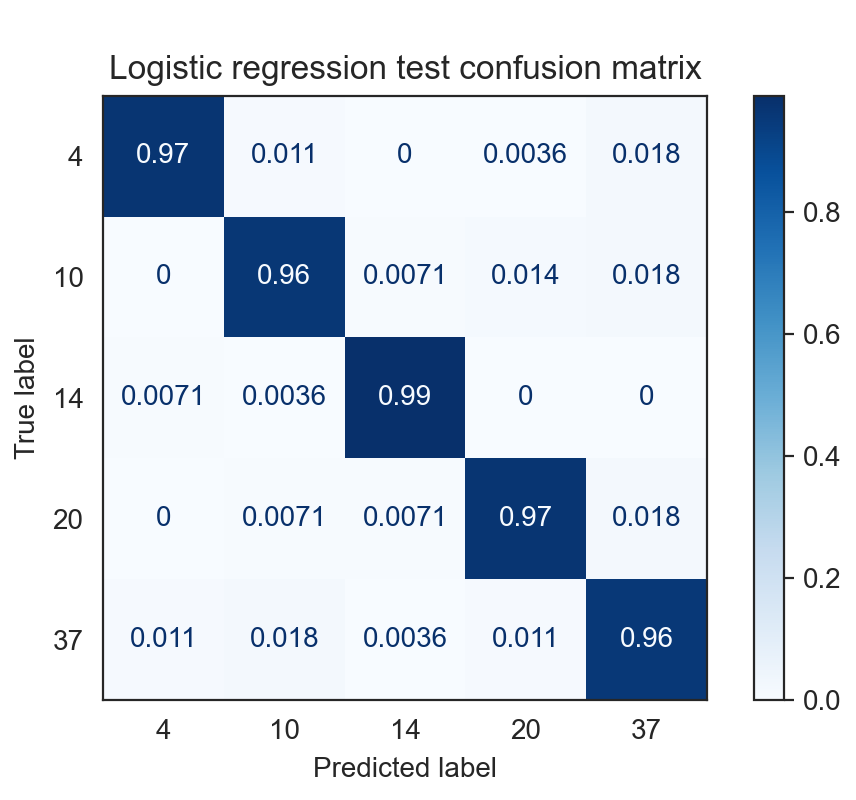
\includegraphics[width=0.8\linewidth]{lr.png}
                \caption{Logistic regression test confusion matrix.}
                \label{fig:lr}
        \end{figure}

        \begin{figure}[H]
                \centering
                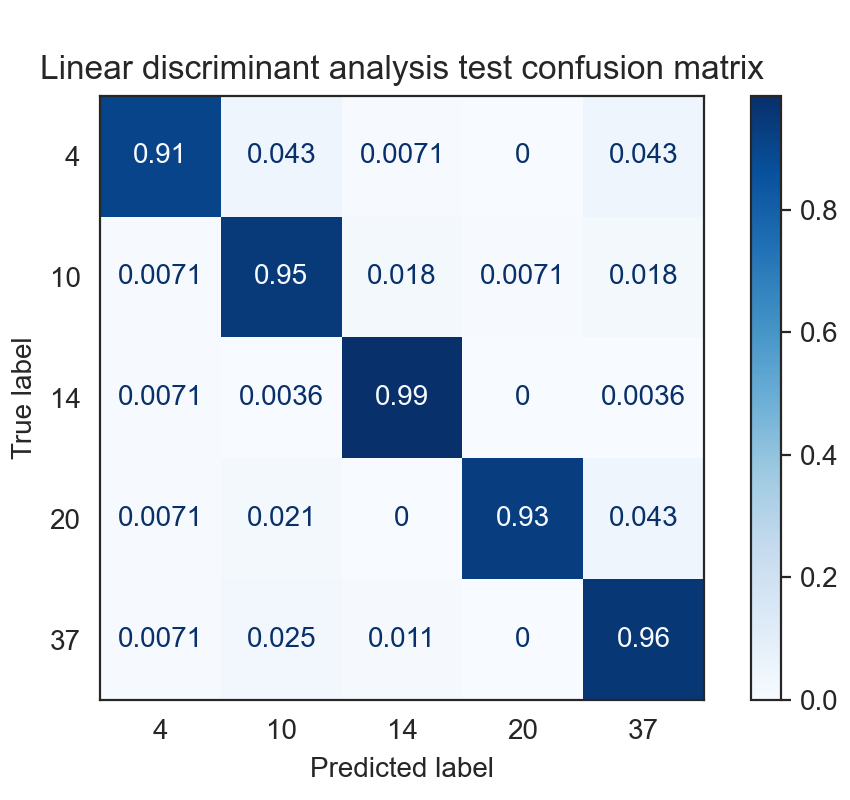
\includegraphics[width=0.8\linewidth]{lda.png}
                \caption{Linear discriminant analysis test confusion matrix.}
                \label{fig:lda}
        \end{figure}

        \begin{figure}[H]
                \centering
                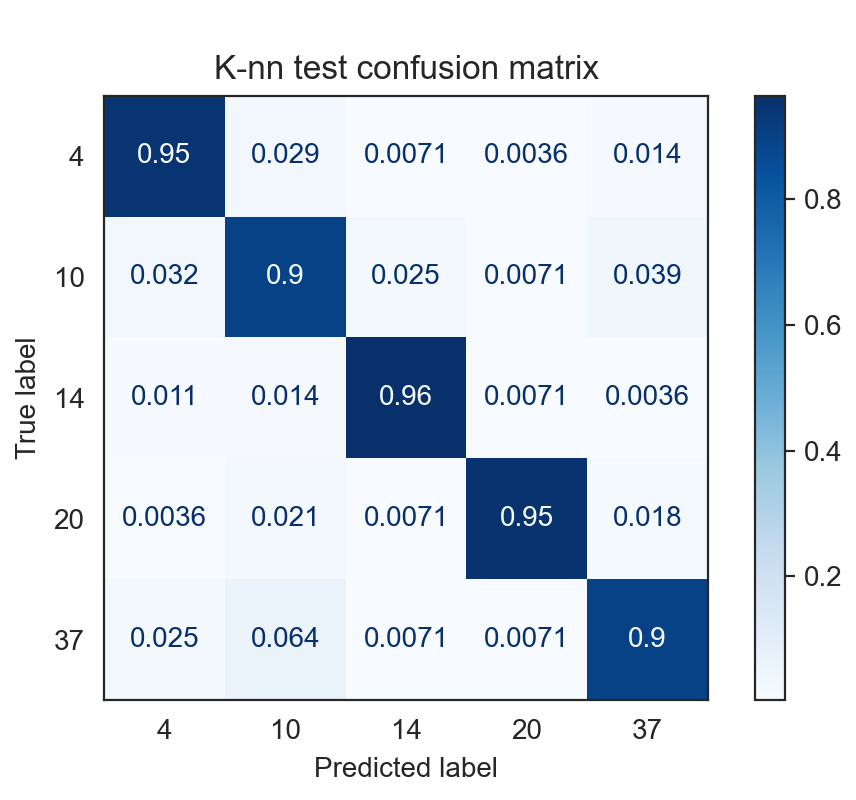
\includegraphics[width=0.8\linewidth]{k_nn.png}
                \caption{K-nearest neighbors test confusion matrix.}
                \label{fig:k_nn}
        \end{figure}

        \begin{figure}[H]
                \centering
                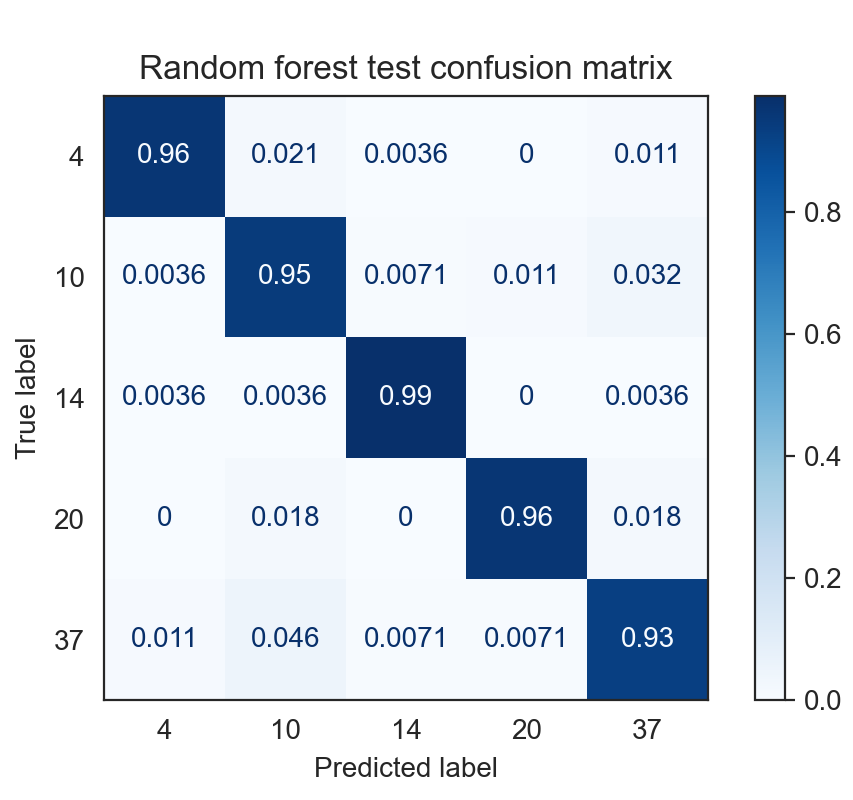
\includegraphics[width=0.8\linewidth]{rf.png}
                \caption{Random forest test confusion matrix.}
                \label{fig:rf}
        \end{figure}

        \begin{figure}[H]
                \centering
                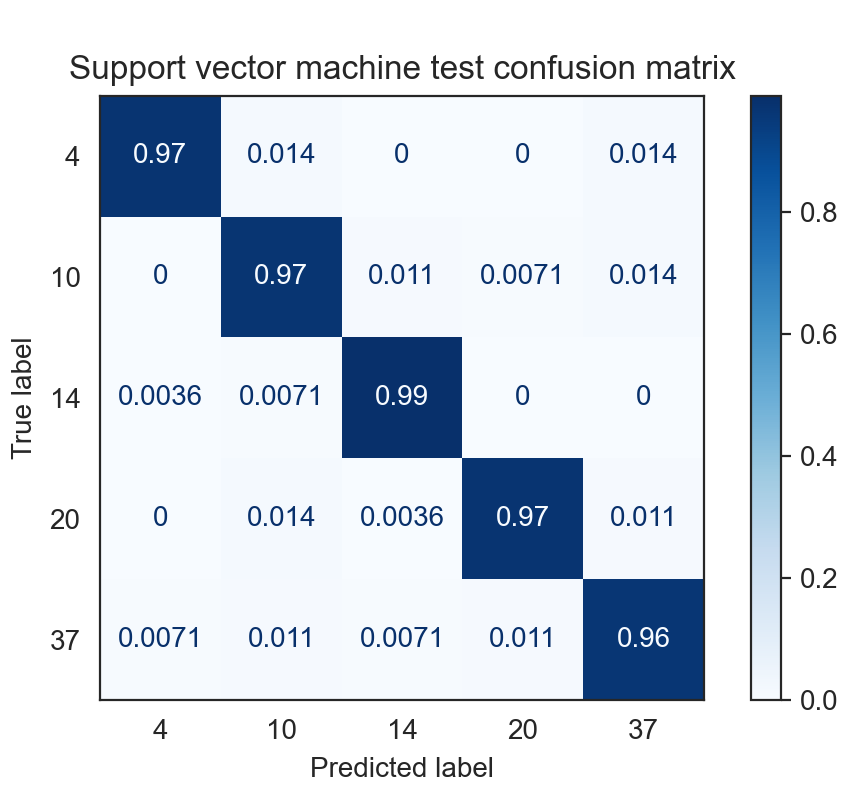
\includegraphics[width=0.8\linewidth]{svm.png}
                \caption{Support vector machine test confusion matrix.}
                \label{fig:svm}
        \end{figure}



      \bibliographystyle{alpha}
      \bibliography{sample}
\end{document}